\documentclass{beamer}

\usepackage[utf8]{inputenc}
\usepackage{graphicx}
\usepackage{tikz}
\usepackage{inconsolata}

\usetheme{Szeged}
\usecolortheme{beaver}

\usepackage{graphicx}
\usepackage[center]{caption}
\usepackage{listings}
\usepackage{xcolor}

\graphicspath{ {../images/} }

\definecolor{dkgreen}{rgb}{0,0.6,0}
\definecolor{gray}{rgb}{0.5,0.5,0.5}
\definecolor{lgray}{rgb}{0.98,0.98,0.98}
\definecolor{mauve}{rgb}{0.58,0,0.82}

\lstset{
	language=Go,
	frame=single,
	aboveskip=1cm,
	belowskip=1cm,
	numbers=none,
	basicstyle=\ttfamily\scriptsize\linespread{1.0},
	backgroundcolor=\color{lgray},
	keywordstyle=\color{blue},
	commentstyle=\color{gray},
	stringstyle=\color{dkgreen},
	showspaces=false,
	showstringspaces=false,
	breakatwhitespace=true,
	captionpos=b,
}

\title{Data Anonymization in Go}
\subtitle{\footnotesize{a practical implementation of an approximation algorithm}}
\titlegraphic{
  
\includegraphics[width=100px]{../images/bme-logo.png}
}

\date{January 2020}
\author{Garai Richárd}
\institute[BME / AUT]{
  \footnotesize{Supervisor: Dr.\ Dudás Ákos} \\[0.5\baselineskip]
  BME / AUT
}

\begin{document}
\frame{\titlepage}

\section{Introduction}

\begin{frame}
  \frametitle{Why do we need anonymization?}
  \begin{columns}
    \column{.6\textwidth}
    \begin{itemize}
      \item{tremendous growth in collection and analysis of personal data\cite{aggarwal}}
        \begin{itemize}
          \item[-]{cloud services}
          \item[-]{mobile apps}
      \item[-]{smart fridge}
      \item[-]{etc\ldots}
        \end{itemize}
      \item{new regulations}
    \begin{itemize}
      \item[-]{EU: GDPR}
        \end{itemize}
    \end{itemize}
    \column{.4\textwidth}
    \begin{figure}
      
\includegraphics{../images/gopher-multimedia.png}
    \end{figure}
  \end{columns}
\end{frame}

\begin{frame}
  \frametitle{Anonymization Concepts}
  \begin{columns}
    \column{.6\textwidth}
    \begin{block}{medical data}
      \vspace{10pt}
      \tiny
      \begin{tabular}{ c|c|c|c|c|c }
        \textbf{name} & \textbf{age} & \textbf{race} & \textbf{gender} & \textbf{zip} & \textbf{disease} \\
        \hline
  \color{orange} John & 47 & white & male & 1077 & \color{violet} cancer \\
        \hline
  \color{orange} Sandy & 35 & white & female & 1077 & \color{violet} flu \\
        \hline
  \color{orange} Mary & 27 & asian & female & 1095 & \color{violet} flu \\
        \hline
  \color{orange} Janet & 27 & white & female & 1095 & \color{violet} hypertension
      \end{tabular}
    \end{block}
    \column{.4\textwidth}
    \begin{itemize}
      \item{\color{orange} identifier}
      \item quasi-identifier
      \item{\color{violet} non-identifier}
    \end{itemize}
  \end{columns}
  \vspace{20pt}
  \begin{columns}
    \column{.6\textwidth}
    \begin{block}{anonymized medical data}
      \vspace{10pt}
      \tiny
        \begin{tabular}{ c|c|c|c|c|c }
        \textbf{name} & \textbf{age} & \textbf{race} & \textbf{gender} & \textbf{zip} & \textbf{disease} \\
        \hline
  \color{red} * & \color{blue} 30..50 & white & \color{red} * & 1077 & cancer \\
        \hline
        \color{red} * & \color{blue} 30..50 & white & \color{red} * & 1077 & flu \\
        \hline
        \color{red} * & 27 & \color{red} * & female & 1095 & flu \\
        \hline
        \color{red} * & 27 & \color{red} * & female & 1095 & hypertension
      \end{tabular}
    \end{block}
    \column{.4\textwidth}
    \begin{itemize}
      \item{\color{red} suppression}
      \item{\color{blue} generalization}
    \end{itemize}
  \end{columns}
\end{frame}

\begin{frame}
  \frametitle{Definition of k-anonymity}
  \begin{block}{k-anonymity}
    \textit{suppress/generalize entries in the table until for each row, there are at least \textcolor{red}{k-1} other rows that are identical to it along the quasi-identifying attributes}
  \end{block}
  \begin{columns}
    \column{.6\textwidth}
    \begin{block}{}
      \begin{itemize}
        \item{k-anonymity even with only suppression and a ternary alphabet, i.e. \(\Sigma = \{0, 1, 2\}\) is NP-hard~\cite{aggarwal} }
      \end{itemize}
    \end{block}
    \column{.4\textwidth}
    \begin{figure}
      
\includegraphics[width=100px]{../images/gopher-calc.png}
    \end{figure}
  \end{columns}
\end{frame}

\section{Algorithm}

\begin{frame}
  \frametitle{Algorithm Outline}
  \begin{enumerate}
    \item Cost Graph Construction
    \item Forest Building
    \item Partition Refinement
  \end{enumerate}
\end{frame}

\begin{frame}
  \frametitle{Cost Graph Construction}
  \begin{columns}
    \column{.5\textwidth}
    \centering
    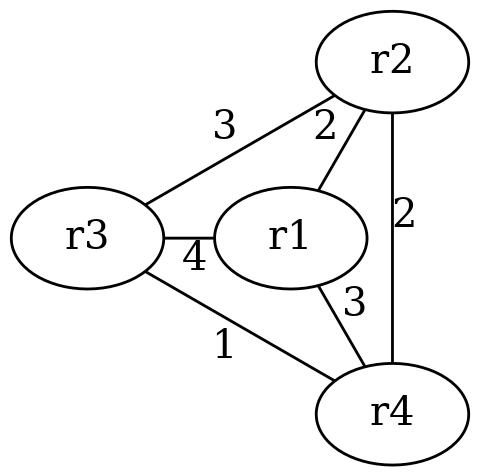
\includegraphics[width=100px]{../graphs/cost-graph.png}
    \column{.5\textwidth}
    \begin{block}{edge weight}
      \(w(e)=\sum_{j}^{} \frac{h_{a,b}(j)}{l_{j}}\) \\
      \scriptsize{
	\textcolor{red}{ \(h_{a,b}\) } generalization cost of items a and b \\
	\textcolor{red}{ \(l_{j}\) } maximum levels of generalization for column j
      }
    \end{block}
  \end{columns}
\end{frame}

\begin{frame}
  \frametitle{Forest Building - Example}
  \begin{columns}
    \column{0.33\textwidth}
    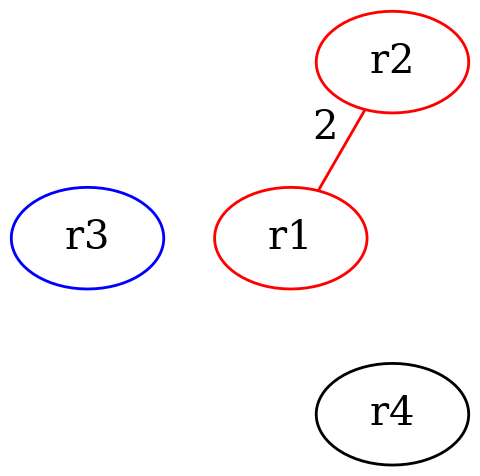
\includegraphics[width=90px]{../graphs/cost-graph-s3.png}
    \column{0.33\textwidth}
    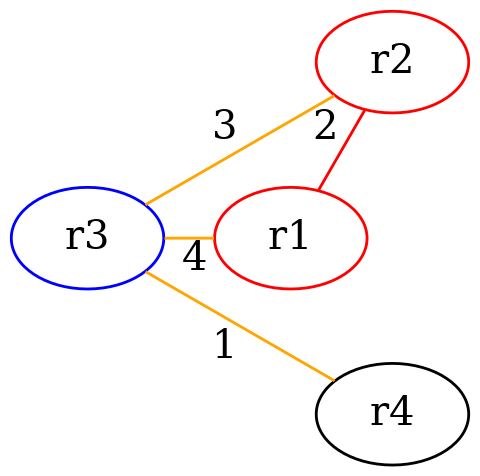
\includegraphics[width=90px]{../graphs/cost-graph-s4.png}
    \column{0.33\textwidth}
    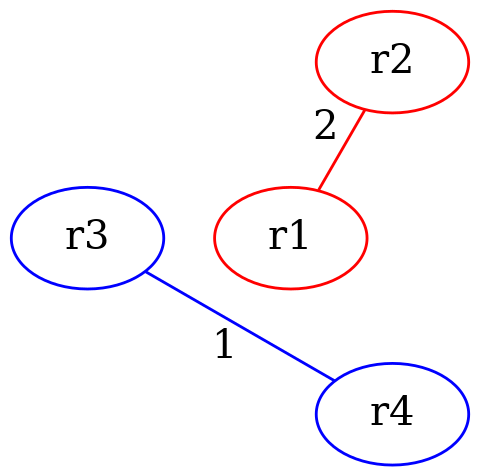
\includegraphics[width=90px]{../graphs/cost-graph-s5.png}
  \end{columns}
\end{frame}

\begin{frame}
  \frametitle{Partition Refinement}
  \begin{columns}
  \column{.6\textwidth}
    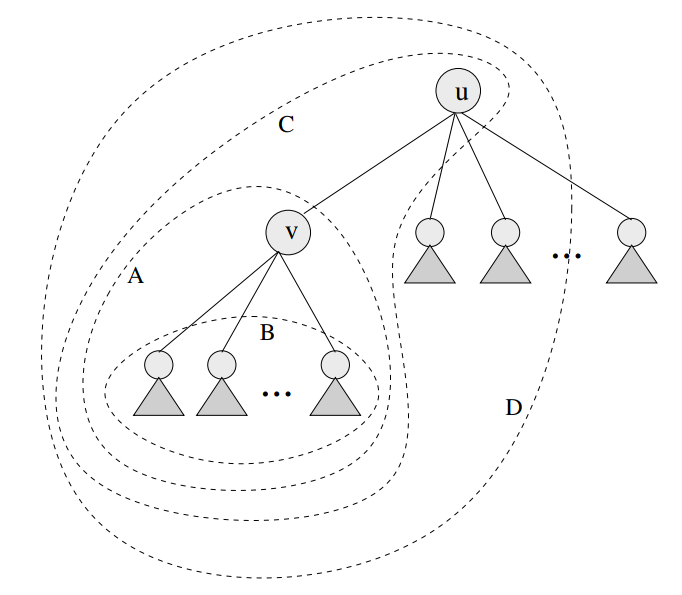
\includegraphics[width=180px]{../images/graph-cuts.png}
  \column{.4\textwidth}
  large components are refined further
  \color{red}\(s > \max\{2k-1,3k-5\}\)
  \begin{itemize}
    \item 4 distinct cut types
    \item  Steiner's Vertices\cite{aggarwal}
  \end{itemize}
  \end{columns}
\end{frame}
\section{Implementation}

\begin{frame}[fragile]
  \frametitle{Code Example}
  \begin{columns}
  \column{.7\textwidth}
  \scriptsize
  \begin{lstlisting}
table := model.NewTable(&model.Schema{
    Columns: []*model.Column{
        model.NewColumn("col1", &gen1),
        model.NewColumn("col2", &gen2),
        // define columns, generalizers
    },
})

table.AddRow(...)   // add rows

a := &Anonymizer{ K: 2, Table: table }
a.Anonymize()
  \end{lstlisting}
  \column{.35\textwidth}
  generalizers:
  \begin{itemize}
    \item suppressor
    \item int range
    \item float range
    \item string prefix
    \item \textcolor{red}{hierarchy}
  \end{itemize}
  \end{columns}
\end{frame}

\section{Performance}

\begin{frame}
    \frametitle{Generalization Benchmarks}
    \centering
    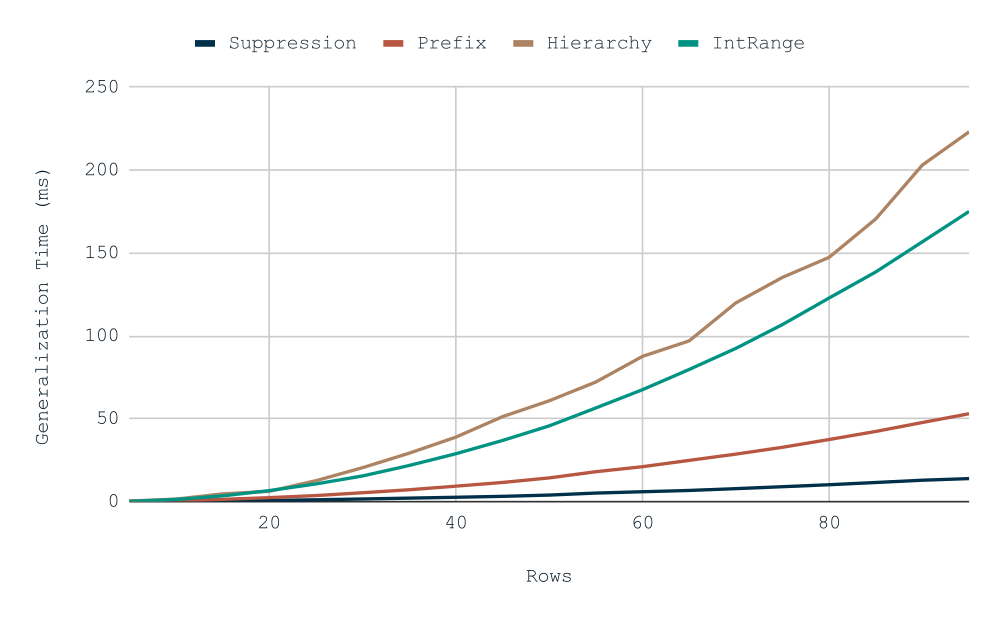
\includegraphics[width=0.9\textwidth]{compare-fast.png}
\end{frame}

\begin{frame}
    \frametitle{Performance --- Row Count}
    \centering
    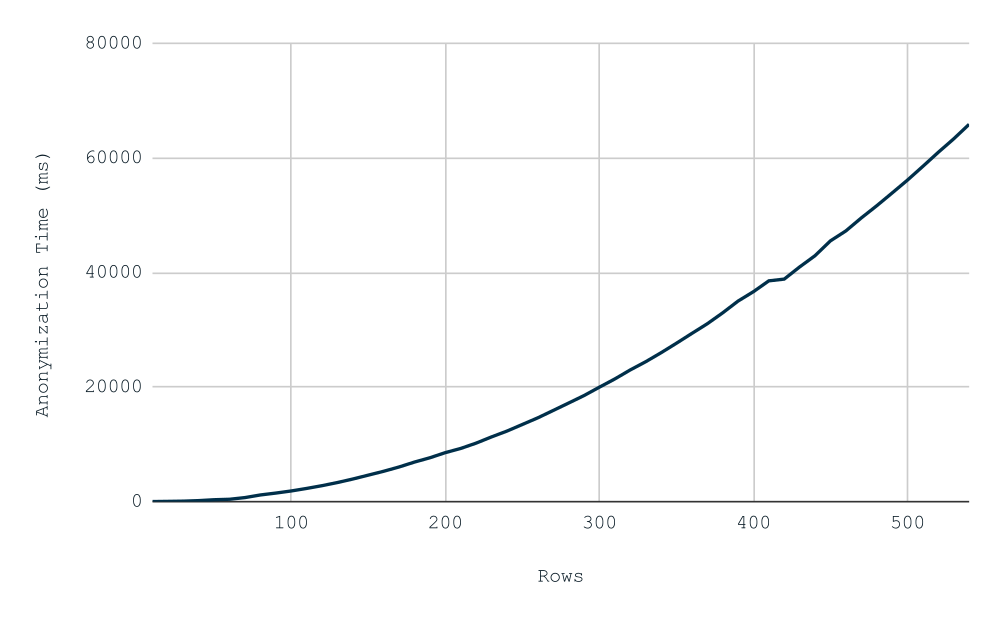
\includegraphics[width=0.9\textwidth]{anon-rows.png}
\end{frame}

\begin{frame}
    \frametitle{Performance --- Column Count}
    \centering
    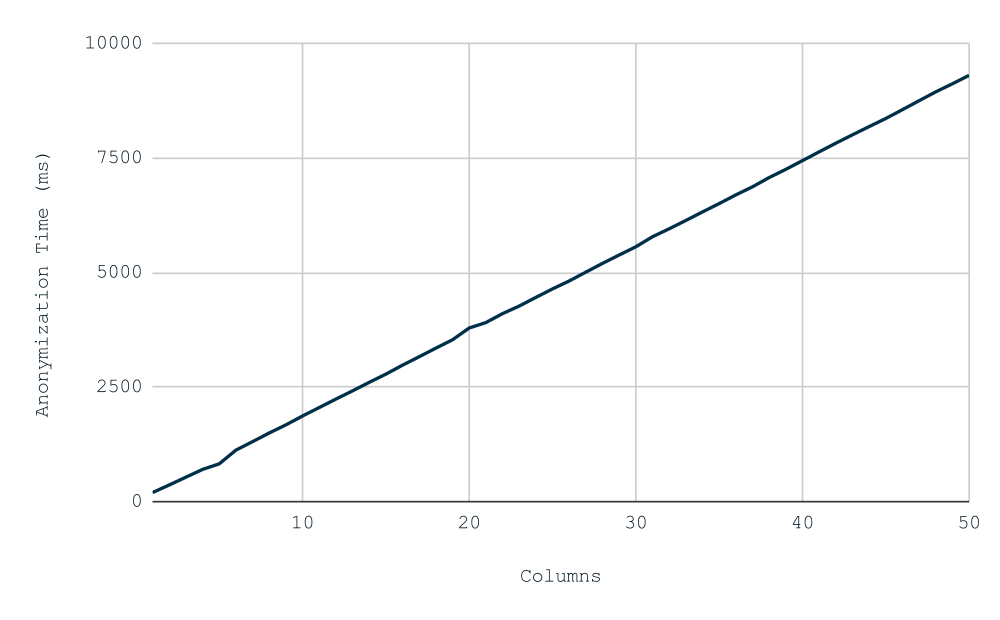
\includegraphics[width=0.9\textwidth]{anon-columns.png}
\end{frame}

\begin{frame}
    \frametitle{Performance --- K value}
    \centering
    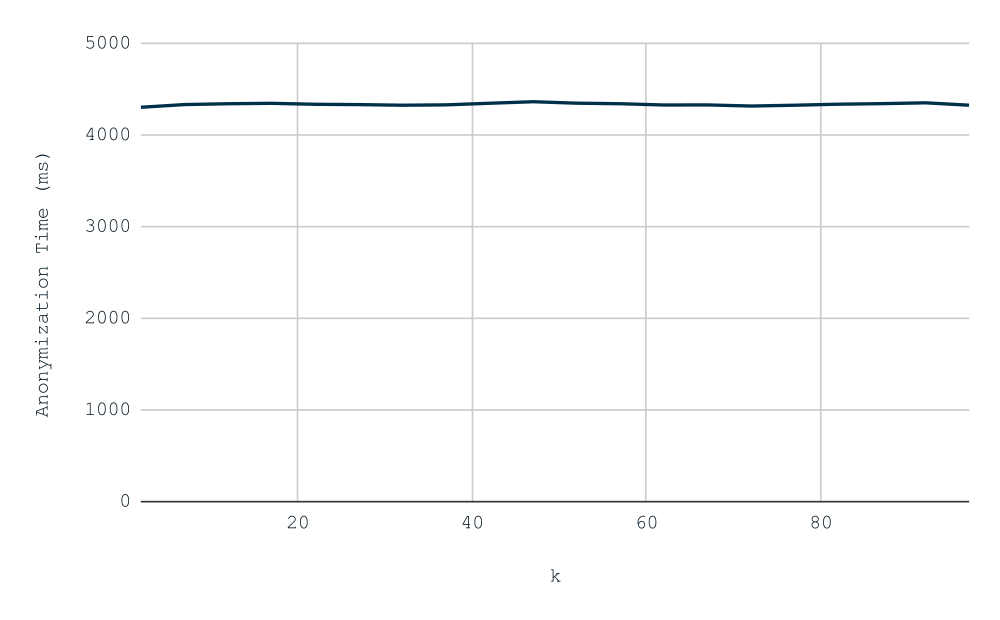
\includegraphics[width=0.9\textwidth]{anon-k.png}
\end{frame}
\section{Closing}

\begin{frame}
    \frametitle{Question 1 --- Heuristics}
    \textit{The algorithm uses random selection when picking the component to extend and the target vertex during the forest building phase.\vspace{\baselineskip}
    What \alert{heuristics} can be used in the above cases, and how can we determine their effectiveness?}
\end{frame}

\begin{frame}
    \frametitle{Answer 1 --- Heuristics}
    \begin{block}{pick source component with smallest/largest size}
    \vspace{10pt}
    \footnotesize
    \centering
    \begin{tabular}{ c|c|c }
        \textbf{rows} & \textbf{smallest} & \textbf{largest} \\
        \hline
        10 & \color{orange}{-0.43\%} & \color{orange}{-38.3\%} \\
        \hline
        20 & \color{dkgreen}{10.55\%} & \color{dkgreen}{2.61\%} \\
        \hline
        30 & \color{orange}{-1.74\%} & \color{dkgreen}{9.57\%} \\
        \hline
        40 & \color{orange}{-2.22\%} & \color{orange}{-1.9\%} \\
        \hline
        50 & \color{orange}{-18.92\%} & \color{orange}{-11.40\%} \\
        \hline
        60 & \color{dkgreen}{3.31\%} & \color{dkgreen}{4.92\%} \\
        \hline
        70 & \color{orange}{-8.1\%} & \color{orange}{-0.29\%} \\
        \hline
        80 & \color{orange}{-0.48\%} & \color{orange}{-0.84\%} \\
        \hline
        90 & \color{dkgreen}{0.99\%} & \color{dkgreen}{1.05\%} \\
        \hline
        100 & \color{dkgreen}{0.11\%} & \color{orange}{-0.09\%} \\
    \end{tabular}
    \end{block}
\end{frame}

\begin{frame}
    \frametitle{Question 2 --- Algorithm Termination}
    \textit{The forest building and partition refinement steps of the algorithm cause the size of components to grow and then shrink respectively.\vspace{\baselineskip}
    What is the proof that \alert{the algorithm terminates} in a finite number of steps?}
\end{frame}

\begin{frame}
    \frametitle{Answer 2 --- Algorithm Termination}
    \begin{columns}
        \column{.6\textwidth}
        \begin{block}{Proof: Forest Building Terminates}
            \begin{itemize}
                \item in each iteration we consider the connected components in the graph
                \item since \(k \le n\) one of the following statements will be true:
                \begin{enumerate}
                    \item at least one component has size \(s < k\)
                    \item every component has size \(s \ge k\) and Forest Building terminates
                \end{enumerate}
            \end{itemize}
        \end{block}
        \column{.4\textwidth}
            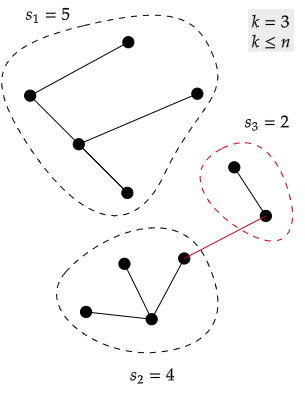
\includegraphics[width=110px]{fb-term.png}
    \end{columns}
\end{frame}

\begin{frame}
    \frametitle{Answer 2 --- Algorithm Termination}
    \begin{block}{Proof: Partition Refinement Terminates}
        \scriptsize{
            in each iteration when finding candidate vertex \(u\), one of the following is true:
            \begin{itemize}
                \item we can apply one of the cut types listed below and the algorithm terminates
                \item we pick the root of the largest subtree \(v\) as the new candidate vertex and the size of the largest subtree \( \phi \) decreases
            \end{itemize}
        }
    \end{block}
    \begin{columns}
        \column{0.5\textwidth}
            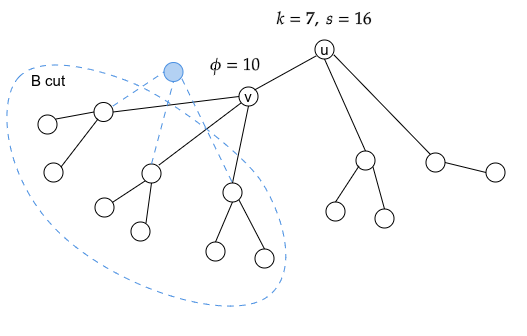
\includegraphics[width=150px]{pr-term.png}
        \column{0.5\textwidth}
            \scriptsize{
                \begin{itemize}
                    \item \alert{Type A}: \( \phi \ge k \) and \(s - \phi \ge k\)
                    \item \alert{Type B}: \( s - \phi = k-1 \)
                    \item \alert{Type C}: \( \phi = k-1 \)
                    \item \alert{Type D}: size of all sub-trees \(\le k-2\)
                \end{itemize}
            }
    \end{columns}
    \scriptsize{\alert{formal proof exists}: \textit{Lemma 4} on page 11 of reference\cite{aggarwal}}
\end{frame}


\begin{frame}
    \frametitle{References}
    \begin{columns}
        \column{.6\textwidth}
            \bibliographystyle{plain}
            \bibliography{../paper/references}
        \column{.4\textwidth}
        
\includegraphics[width=120px]{gophers.png}
    \end{columns}
\end{frame}




\end{document}